\subsection{Agentic Search}


Single-agent Agentic Retrieval-Augmented Generation (RAG) systems embed reasoning and control into a centralized agent that governs the entire retrieval-generation loop.
Unlike traditional RAG pipelines~\cite{lewis2020retrieval, huang2024survey, yang2024crag} that perform fixed, one-shot retrieval before generation, agentic RAG agents dynamically control \textit{when}, \textit{what}, and \textit{how} to retrieve based on real-time reasoning needs. This enables the model to adapt retrieval strategies mid-inference, refine its queries, and better integrate evidence from multiple sources. Based on how the agent selects, refines, and integrates retrieved content during reasoning, we categorize single-agent Agentic RAG systems into three distinct architectural styles: \textit{in-context}, \textit{post-training}, and \textit{structure-enhanced} agentic RAG.  

\begin{figure}
    \centering
    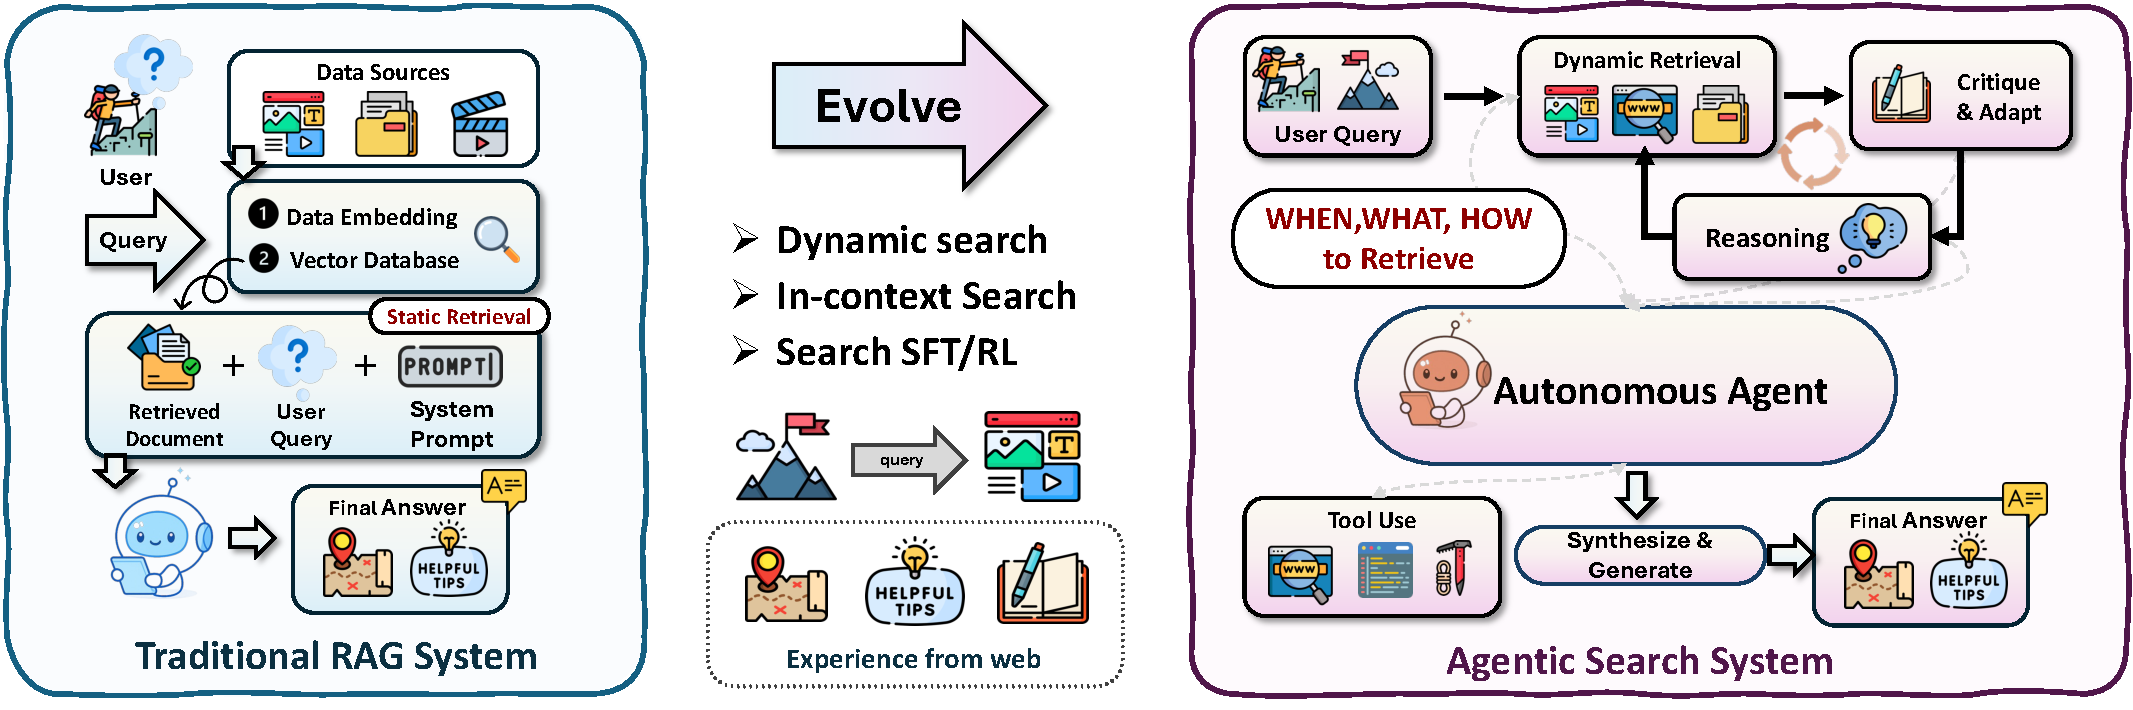
\includegraphics[width=\linewidth]{arxiv/figs/Agentic_search.pdf}
    \caption{Comparison between \textbf{traditional RAG} systems and \textbf{agentic search} systems. Traditional RAG relies on static retrieval over a vector database, while agentic search introduces autonomous decision-making for when, what, and how to retrieve, enabling dynamic search, in-context retrieval, critique-and-adapt loops, and tool use.}
    \label{fig:agentic_rag}
\end{figure}


\begin{table*}[!t]
\centering
\caption{
Representative \textbf{Agentic Search} systems categorized by \textit{Reasoning Structure}, \textit{Format}, and \textit{Tool Use}. 
{NL} denotes natural language traces used during reasoning, {Ops} refers to symbolic or graph operations, and {KG} stands for knowledge graph. 
Tool use includes search APIs, browser actions, or KG-based retrieval.
}
\renewcommand{\arraystretch}{1.15}
\setlength{\tabcolsep}{6pt}
\begin{tabular}{p{3cm}>{\centering\arraybackslash}p{3cm}>{\centering\arraybackslash}p{4cm}>{\centering\arraybackslash}p{5.5cm}}
\toprule
\textbf{Method} & \textbf{Structure} & \textbf{Format} & \textbf{Tool} \\
\midrule
\rowcolor[HTML]{F5F5F5}
\multicolumn{4}{l}{\textbf{Modality I: In-Context Agentic Search}} \\
ReAct~\cite{yao2023react} & Interleaved & NL + Actions & Search API \\
Self-Ask~\cite{press2022measuring} & Decomposed & NL Queries & Search API \\
IRCoT~\cite{trivedi2022interleaving} & Sequential & NL + CoT & Search API \\
Self-RAG~\cite{asai2023self} & Reflective & NL Self-check & Conditional Search \\
DeepRAG~\cite{guan2025deeprag} & Iterative & NL Feedback & Search API \\
\midrule
\rowcolor[HTML]{F5F5F5}
\multicolumn{4}{l}{\textbf{Modality II: Post-Training Agentic Search}} \\
Toolformer~\cite{schick2023toolformer} & Sequential & Tool Tokens & APIs, Search \\
INTERS~\cite{zhu2024inters} & Sequential & Instructions & Search API \\
WebGPT~\cite{nakano2021webgpt} & Sequential & NL + Browser & Web Search \\
RAG-RL~\cite{huang2025rag} & Decision & NL Policy & Evidence API \\
Search\text{-}R1~\cite{jin2025search} & Iterative & NL + Tokens & Live Web \\
Deep-Researcher~\cite{zheng2025deepresearcher} & Multi-step & NL Trajectories & Browser Tools \\
ReSearch~\cite{chen2025learning} & Step-wise & NL Steps & Search + Verifier \\
ReARTeR~\cite{sun2025rearter} & Reflective & NL Policy & Tool Cluster \\
\midrule
\rowcolor[HTML]{F5F5F5}
\multicolumn{4}{l}{\textbf{Modality III: Structure-Enhanced Agentic Search}} \\
Agent\text{-}G~\cite{leeagent} & Modular & NL + Graph Ops & KG Query \\
MC-Search~\cite{ning2025mc} & Multi-step & NL & Multimodal Search \\
GeAR~\cite{shen2025gear} & Graph & Graph Ops & KG Expansion \\
ARG~\cite{zhang2025learning} & Reflective & NL + Symbols & KG Traversal \\
\bottomrule
\end{tabular}
\label{tab:agentic_search_methods}
\end{table*}



\subsubsection{In-Context Search}

\paragraph{Interleaving Reasoning and Search.}

In-context agentic RAG systems embed retrieval behavior directly into the inference process of language models through carefully designed prompting strategies. Rather than training the model to learn retrieval behavior, these methods guide it to alternate between reasoning and search within a single forward pass, typically via few-shot exemplars or special tokens. A representative example is ReAct~\cite{yao2023react}, which interleaves Chain-of-Thought reasoning with tool-use commands such as \texttt{<Search>} to dynamically invoke external APIs or knowledge sources. Extensions such as Self-Ask~\cite{press2022measuring} and IRCoT~\cite{trivedi2022interleaving} go beyond sequential reasoning by prompting the model to recursively decompose questions and retrieve sub-evidence accordingly. More recent methods~\cite{asai2023self, li2024benchmarking, guan2025deeprag, ning2025mc} introduce reflective retrieval, where the model explicitly assesses whether it needs additional information at each step, deciding to retrieve only when necessary. These approaches require no additional training, making them highly flexible and deployable, but often rely on prompt engineering and may struggle with stability across diverse domains.

\paragraph{Structure-Enhanced Search.}

Structure-enhanced agentic RAG systems enhance retrieval-augmented generation by enabling a single agent to reason over symbolic knowledge sources such as knowledge graphs through dynamic querying, tool invocation, and reflective self-monitoring. Unlike static KG retrievers or query executors, these agents decide when to access structured knowledge, how to formulate graph-based queries, and whether retrieved information suffices for continuing the reasoning trajectory. Agent-G~\cite{leeagent} introduces a modular agentic architecture that integrates unstructured document retrieval with structured graph reasoning, using feedback loops and specialized retriever modules to ensure accurate multi-hop responses. MC-Search~\cite{ning2025mc} introduces five canonical reasoning topologies to model multimodal search-enhanced reasoning process, and proposes a end-to-end agentic RAG and step-wise evaluation pipeline to evaluate model's planning and retrieval fidelity across heterogeneous sources. Similarly, GeAR~\cite{shen2025gear} incorporates graph expansion operations into an agentic controller to address challenges in complex multi-hop queries, enhancing coherence across structured and unstructured sources. Beyond retrieval orchestration, ARG~\cite{zhang2025learning} proposes a fully end-to-end agentic framework for reasoning over knowledge graphs via active self-reflection. The model autonomously determines when to retrieve, performs iterative critique based on symbolic inputs, and exhibits interpretable, step-wise reasoning behavior over graphs. Together, these systems represent a shift from passive graph access to active, feedback-driven symbolic reasoning, highlighting the potential of structured agentic RAG to achieve both factual reliability and interpretability.

\subsubsection{Post-Training Search}
Post-training agentic RAG methods endow language models with retrieval-aware capabilities by fine-tuning them to make informed decisions throughout multi-step reasoning. Unlike in-context prompting, these approaches train models, either via supervised fine-tuning (SFT) or reinforcement learning (RL), to determine when retrieval is necessary, how to formulate queries, and how to incorporate retrieved evidence.

\paragraph{SFT-Based Agentic Search.} These methods construct curated or synthetic datasets that interleave retrieval operations with natural language reasoning, and subsequently apply supervised fine-tuning to instill retrieval-aware capabilities into the model. Toolformer~\cite{schick2023toolformer} introduces a self-supervised approach to annotate tool-use behaviors within model-generated text, enabling LLMs to learn when and how to invoke tools such as web search or calculators. INTERS~\cite{zhu2024inters} extends this direction by performing instruction-based fine-tuning over a diverse, multi-task dataset compiled from over 40 sources, capturing a wide spectrum of retrieval-reasoning patterns. This class of methods benefits from scalable data generation pipelines~\cite{mao2024rag, zhang2024raft, li2025search}, which minimize the need for human annotation. Instructional reformulation techniques~\cite{lin2023ra,zhu2024inters, nguyen2024sfr} further enhance generalization by aligning tasks with human-preferred formats and reasoning.

\paragraph{RL-Based Agentic Search.} These methods optimize retrieval-aware behaviors through reward signals that reflect answer quality, factuality, or user preferences. WebGPT~\cite{nakano2021webgpt} introduces reward modeling to supervise search-augmented chains aligned with human judgment, while RAG-RL~\cite{huang2025rag} formulates retrieval as a sequential decision-making task over evidence access. More recent efforts such as Search-R1~\cite{jin2025search} and Deep-Researcher~\cite{zheng2025deepresearcher} go further by training agents to dynamically issue retrieval actions (e.g., generating \texttt{<Search>} tokens mid-reasoning) and operate in open-ended environments such as the live web. These agents exhibit emergent capabilities such as iterative decomposition, re-verification, and evidence planning. Finally, systems like ReSearch~\cite{chen2025learning} and ReARTeR~\cite{sun2025rearter} pursue not only accurate answers but also interpretable and faithful reasoning trajectories, highlighting the potential of reinforcement-learned retrievers to act as controllable and reflective agents.

